% Created by tikzDevice version 0.12.6 on 2026-08-16 23:27:46
% !TEX encoding = UTF-8 Unicode
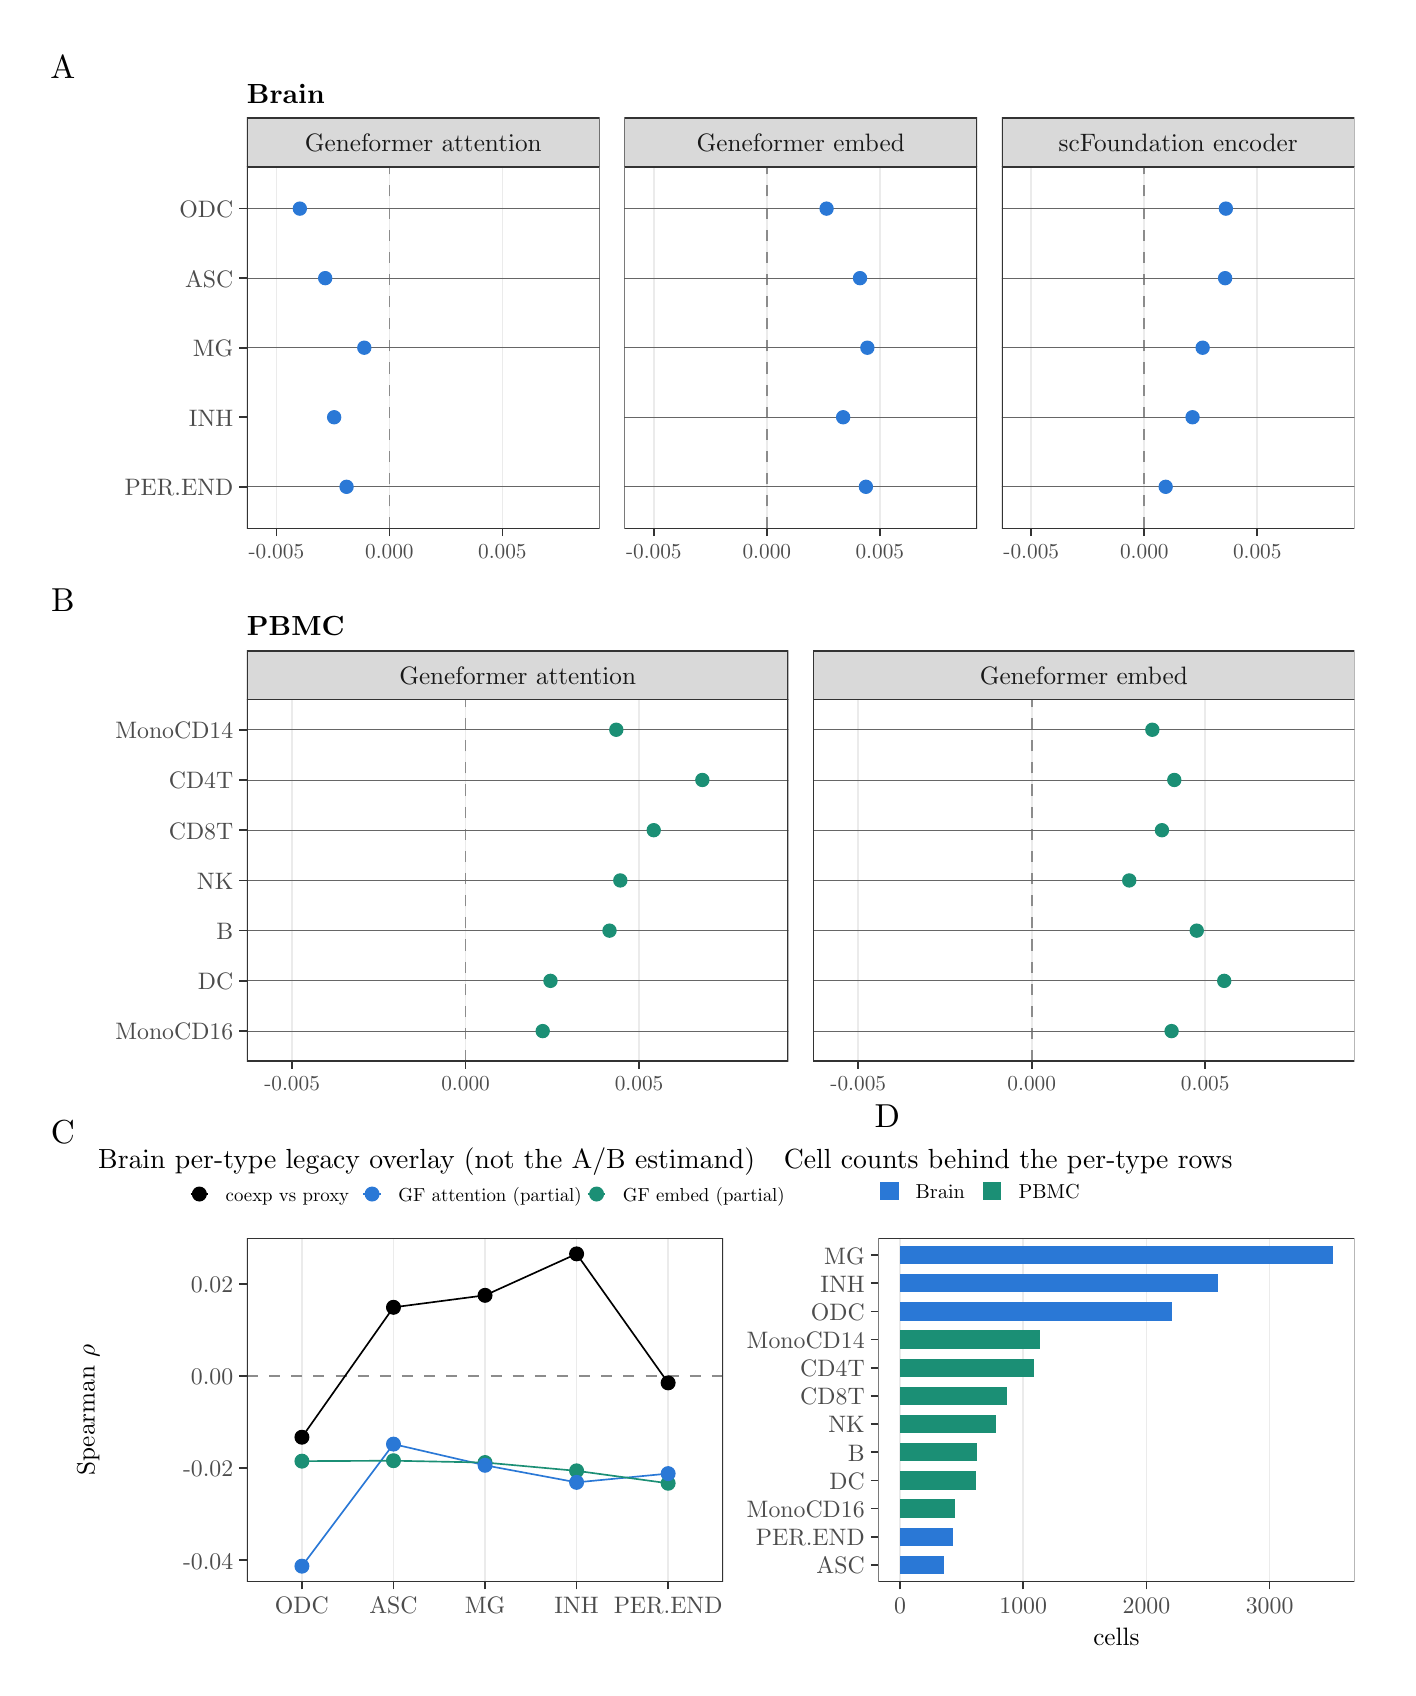
\begin{tikzpicture}[x=1pt,y=1pt]
\definecolor{fillColor}{RGB}{255,255,255}
\path[use as bounding box,fill=fillColor,fill opacity=0.00] (0,0) rectangle (491.44,592.61);
\begin{scope}
\path[clip] (  0.00,  0.00) rectangle (491.44,592.61);
\definecolor{drawColor}{RGB}{255,255,255}
\definecolor{fillColor}{RGB}{255,255,255}

\path[draw=drawColor,line width= 0.6pt,line join=round,line cap=round,fill=fillColor] ( -0.00, -0.00) rectangle (491.44,592.61);
\end{scope}
\begin{scope}
\path[clip] (  4.00,396.12) rectangle (485.44,588.61);
\definecolor{drawColor}{RGB}{255,255,255}
\definecolor{fillColor}{RGB}{255,255,255}

\path[draw=drawColor,line width= 0.6pt,line join=round,line cap=round,fill=fillColor] (  4.00,396.12) rectangle (485.44,588.61);
\end{scope}
\begin{scope}
\path[clip] (  4.00,203.63) rectangle (485.44,396.12);
\definecolor{drawColor}{RGB}{255,255,255}
\definecolor{fillColor}{RGB}{255,255,255}

\path[draw=drawColor,line width= 0.6pt,line join=round,line cap=round,fill=fillColor] (  4.00,203.63) rectangle (485.44,396.12);
\end{scope}
\begin{scope}
\path[clip] ( 79.25,411.62) rectangle (206.65,542.29);
\definecolor{fillColor}{RGB}{255,255,255}

\path[fill=fillColor] ( 79.25,411.62) rectangle (206.65,542.29);
\definecolor{drawColor}{gray}{0.92}

\path[draw=drawColor,line width= 0.6pt,line join=round] ( 89.87,411.62) --
	( 89.87,542.29);

\path[draw=drawColor,line width= 0.6pt,line join=round] (130.70,411.62) --
	(130.70,542.29);

\path[draw=drawColor,line width= 0.6pt,line join=round] (171.53,411.62) --
	(171.53,542.29);
\definecolor{drawColor}{gray}{0.55}

\path[draw=drawColor,line width= 0.6pt,dash pattern=on 4pt off 4pt ,line join=round] (130.70,411.62) -- (130.70,542.29);
\definecolor{drawColor}{gray}{0.40}

\path[draw=drawColor,line width= 0.3pt,line join=round] (343.84,524.07) --
	(343.84,530.36);

\path[draw=drawColor,line width= 0.3pt,line join=round] (343.84,527.22) --
	(-1151.40,527.22);

\path[draw=drawColor,line width= 0.3pt,line join=round] (-1151.40,524.07) --
	(-1151.40,530.36);

\path[draw=drawColor,line width= 0.3pt,line join=round] (498.18,498.95) --
	(498.18,505.23);

\path[draw=drawColor,line width= 0.3pt,line join=round] (498.18,502.09) --
	(-981.54,502.09);

\path[draw=drawColor,line width= 0.3pt,line join=round] (-981.54,498.95) --
	(-981.54,505.23);

\path[draw=drawColor,line width= 0.3pt,line join=round] (717.86,473.82) --
	(717.86,480.10);

\path[draw=drawColor,line width= 0.3pt,line join=round] (717.86,476.96) --
	(-802.70,476.96);

\path[draw=drawColor,line width= 0.3pt,line join=round] (-802.70,473.82) --
	(-802.70,480.10);

\path[draw=drawColor,line width= 0.3pt,line join=round] (-146.13,448.69) --
	(-146.13,454.97);

\path[draw=drawColor,line width= 0.3pt,line join=round] (-146.13,451.83) --
	(-1576.87,451.83);

\path[draw=drawColor,line width= 0.3pt,line join=round] (-1576.87,448.69) --
	(-1576.87,454.97);

\path[draw=drawColor,line width= 0.3pt,line join=round] (231.96,423.56) --
	(231.96,429.84);

\path[draw=drawColor,line width= 0.3pt,line join=round] (231.96,426.70) --
	(-1267.36,426.70);

\path[draw=drawColor,line width= 0.3pt,line join=round] (-1267.36,423.56) --
	(-1267.36,429.84);
\definecolor{drawColor}{RGB}{42,120,214}
\definecolor{fillColor}{RGB}{42,120,214}

\path[draw=drawColor,line width= 0.4pt,line join=round,line cap=round,fill=fillColor] ( 98.34,527.22) circle (  2.39);

\path[draw=drawColor,line width= 0.4pt,line join=round,line cap=round,fill=fillColor] (107.51,502.09) circle (  2.39);

\path[draw=drawColor,line width= 0.4pt,line join=round,line cap=round,fill=fillColor] (121.64,476.96) circle (  2.39);

\path[draw=drawColor,line width= 0.4pt,line join=round,line cap=round,fill=fillColor] (110.74,451.83) circle (  2.39);

\path[draw=drawColor,line width= 0.4pt,line join=round,line cap=round,fill=fillColor] (115.23,426.70) circle (  2.39);
\definecolor{drawColor}{gray}{0.20}

\path[draw=drawColor,line width= 0.6pt,line join=round,line cap=round] ( 79.25,411.62) rectangle (206.65,542.29);
\end{scope}
\begin{scope}
\path[clip] (215.65,411.62) rectangle (343.04,542.29);
\definecolor{fillColor}{RGB}{255,255,255}

\path[fill=fillColor] (215.65,411.62) rectangle (343.04,542.29);
\definecolor{drawColor}{gray}{0.92}

\path[draw=drawColor,line width= 0.6pt,line join=round] (226.26,411.62) --
	(226.26,542.29);

\path[draw=drawColor,line width= 0.6pt,line join=round] (267.10,411.62) --
	(267.10,542.29);

\path[draw=drawColor,line width= 0.6pt,line join=round] (307.93,411.62) --
	(307.93,542.29);
\definecolor{drawColor}{gray}{0.55}

\path[draw=drawColor,line width= 0.6pt,dash pattern=on 4pt off 4pt ,line join=round] (267.10,411.62) -- (267.10,542.29);
\definecolor{drawColor}{gray}{0.40}

\path[draw=drawColor,line width= 0.3pt,line join=round] (927.75,524.07) --
	(927.75,530.36);

\path[draw=drawColor,line width= 0.3pt,line join=round] (927.75,527.22) --
	(-574.85,527.22);

\path[draw=drawColor,line width= 0.3pt,line join=round] (-574.85,524.07) --
	(-574.85,530.36);

\path[draw=drawColor,line width= 0.3pt,line join=round] (1198.87,498.95) --
	(1198.87,505.23);

\path[draw=drawColor,line width= 0.3pt,line join=round] (1198.87,502.09) --
	(-304.54,502.09);

\path[draw=drawColor,line width= 0.3pt,line join=round] (-304.54,498.95) --
	(-304.54,505.23);

\path[draw=drawColor,line width= 0.3pt,line join=round] (1198.05,473.82) --
	(1198.05,480.10);

\path[draw=drawColor,line width= 0.3pt,line join=round] (1198.05,476.96) --
	(-347.82,476.96);

\path[draw=drawColor,line width= 0.3pt,line join=round] (-347.82,473.82) --
	(-347.82,480.10);

\path[draw=drawColor,line width= 0.3pt,line join=round] (1224.18,448.69) --
	(1224.18,454.97);

\path[draw=drawColor,line width= 0.3pt,line join=round] (1224.18,451.83) --
	(-240.03,451.83);

\path[draw=drawColor,line width= 0.3pt,line join=round] (-240.03,448.69) --
	(-240.03,454.97);

\path[draw=drawColor,line width= 0.3pt,line join=round] (1033.09,423.56) --
	(1033.09,429.84);

\path[draw=drawColor,line width= 0.3pt,line join=round] (1033.09,426.70) --
	(-440.10,426.70);

\path[draw=drawColor,line width= 0.3pt,line join=round] (-440.10,423.56) --
	(-440.10,429.84);
\definecolor{drawColor}{RGB}{42,120,214}
\definecolor{fillColor}{RGB}{42,120,214}

\path[draw=drawColor,line width= 0.4pt,line join=round,line cap=round,fill=fillColor] (288.68,527.22) circle (  2.39);

\path[draw=drawColor,line width= 0.4pt,line join=round,line cap=round,fill=fillColor] (300.76,502.09) circle (  2.39);

\path[draw=drawColor,line width= 0.4pt,line join=round,line cap=round,fill=fillColor] (303.42,476.96) circle (  2.39);

\path[draw=drawColor,line width= 0.4pt,line join=round,line cap=round,fill=fillColor] (294.67,451.83) circle (  2.39);

\path[draw=drawColor,line width= 0.4pt,line join=round,line cap=round,fill=fillColor] (302.89,426.70) circle (  2.39);
\definecolor{drawColor}{gray}{0.20}

\path[draw=drawColor,line width= 0.6pt,line join=round,line cap=round] (215.65,411.62) rectangle (343.04,542.29);
\end{scope}
\begin{scope}
\path[clip] (352.04,411.62) rectangle (479.44,542.29);
\definecolor{fillColor}{RGB}{255,255,255}

\path[fill=fillColor] (352.04,411.62) rectangle (479.44,542.29);
\definecolor{drawColor}{gray}{0.92}

\path[draw=drawColor,line width= 0.6pt,line join=round] (362.66,411.62) --
	(362.66,542.29);

\path[draw=drawColor,line width= 0.6pt,line join=round] (403.49,411.62) --
	(403.49,542.29);

\path[draw=drawColor,line width= 0.6pt,line join=round] (444.32,411.62) --
	(444.32,542.29);
\definecolor{drawColor}{gray}{0.55}

\path[draw=drawColor,line width= 0.6pt,dash pattern=on 4pt off 4pt ,line join=round] (403.49,411.62) -- (403.49,542.29);
\definecolor{drawColor}{gray}{0.40}

\path[draw=drawColor,line width= 0.3pt,line join=round] (982.48,524.07) --
	(982.48,530.36);

\path[draw=drawColor,line width= 0.3pt,line join=round] (982.48,527.22) --
	(-605.05,527.22);

\path[draw=drawColor,line width= 0.3pt,line join=round] (-605.05,524.07) --
	(-605.05,530.36);

\path[draw=drawColor,line width= 0.3pt,line join=round] (1344.24,498.95) --
	(1344.24,505.23);

\path[draw=drawColor,line width= 0.3pt,line join=round] (1344.24,502.09) --
	(-171.42,502.09);

\path[draw=drawColor,line width= 0.3pt,line join=round] (-171.42,498.95) --
	(-171.42,505.23);

\path[draw=drawColor,line width= 0.3pt,line join=round] (1389.98,473.82) --
	(1389.98,480.10);

\path[draw=drawColor,line width= 0.3pt,line join=round] (1389.98,476.96) --
	(-129.77,476.96);

\path[draw=drawColor,line width= 0.3pt,line join=round] (-129.77,473.82) --
	(-129.77,480.10);

\path[draw=drawColor,line width= 0.3pt,line join=round] (1117.22,448.69) --
	(1117.22,454.97);

\path[draw=drawColor,line width= 0.3pt,line join=round] (1117.22,451.83) --
	(-329.03,451.83);

\path[draw=drawColor,line width= 0.3pt,line join=round] (-329.03,448.69) --
	(-329.03,454.97);

\path[draw=drawColor,line width= 0.3pt,line join=round] (1552.48,423.56) --
	(1552.48,429.84);

\path[draw=drawColor,line width= 0.3pt,line join=round] (1552.48,426.70) --
	( 51.52,426.70);

\path[draw=drawColor,line width= 0.3pt,line join=round] ( 51.52,423.56) --
	( 51.52,429.84);
\definecolor{drawColor}{RGB}{42,120,214}
\definecolor{fillColor}{RGB}{42,120,214}

\path[draw=drawColor,line width= 0.4pt,line join=round,line cap=round,fill=fillColor] (432.97,527.22) circle (  2.39);

\path[draw=drawColor,line width= 0.4pt,line join=round,line cap=round,fill=fillColor] (432.69,502.09) circle (  2.39);

\path[draw=drawColor,line width= 0.4pt,line join=round,line cap=round,fill=fillColor] (424.57,476.96) circle (  2.39);

\path[draw=drawColor,line width= 0.4pt,line join=round,line cap=round,fill=fillColor] (420.92,451.83) circle (  2.39);

\path[draw=drawColor,line width= 0.4pt,line join=round,line cap=round,fill=fillColor] (411.21,426.70) circle (  2.39);
\definecolor{drawColor}{gray}{0.20}

\path[draw=drawColor,line width= 0.6pt,line join=round,line cap=round] (352.04,411.62) rectangle (479.44,542.29);
\end{scope}
\begin{scope}
\path[clip] ( 79.25,542.29) rectangle (206.65,559.98);
\definecolor{drawColor}{gray}{0.20}
\definecolor{fillColor}{gray}{0.85}

\path[draw=drawColor,line width= 0.6pt,line join=round,line cap=round,fill=fillColor] ( 79.25,542.29) rectangle (206.65,559.98);
\definecolor{drawColor}{gray}{0.10}

\node[text=drawColor,anchor=base,inner sep=0pt, outer sep=0pt, scale=  0.91] at (142.95,547.77) {Geneformer attention};
\end{scope}
\begin{scope}
\path[clip] (215.65,542.29) rectangle (343.04,559.98);
\definecolor{drawColor}{gray}{0.20}
\definecolor{fillColor}{gray}{0.85}

\path[draw=drawColor,line width= 0.6pt,line join=round,line cap=round,fill=fillColor] (215.65,542.29) rectangle (343.04,559.98);
\definecolor{drawColor}{gray}{0.10}

\node[text=drawColor,anchor=base,inner sep=0pt, outer sep=0pt, scale=  0.91] at (279.35,547.77) {Geneformer embed};
\end{scope}
\begin{scope}
\path[clip] (352.04,542.29) rectangle (479.44,559.98);
\definecolor{drawColor}{gray}{0.20}
\definecolor{fillColor}{gray}{0.85}

\path[draw=drawColor,line width= 0.6pt,line join=round,line cap=round,fill=fillColor] (352.04,542.29) rectangle (479.44,559.98);
\definecolor{drawColor}{gray}{0.10}

\node[text=drawColor,anchor=base,inner sep=0pt, outer sep=0pt, scale=  0.91] at (415.74,547.77) {scFoundation encoder};
\end{scope}
\begin{scope}
\path[clip] (  0.00,  0.00) rectangle (491.44,592.61);
\definecolor{drawColor}{gray}{0.20}

\path[draw=drawColor,line width= 0.6pt,line join=round] ( 89.87,408.87) --
	( 89.87,411.62);

\path[draw=drawColor,line width= 0.6pt,line join=round] (130.70,408.87) --
	(130.70,411.62);

\path[draw=drawColor,line width= 0.6pt,line join=round] (171.53,408.87) --
	(171.53,411.62);
\end{scope}
\begin{scope}
\path[clip] (  0.00,  0.00) rectangle (491.44,592.61);
\definecolor{drawColor}{gray}{0.30}

\node[text=drawColor,anchor=base,inner sep=0pt, outer sep=0pt, scale=  0.77] at ( 89.87,400.95) {-0.005};

\node[text=drawColor,anchor=base,inner sep=0pt, outer sep=0pt, scale=  0.77] at (130.70,400.95) {0.000};

\node[text=drawColor,anchor=base,inner sep=0pt, outer sep=0pt, scale=  0.77] at (171.53,400.95) {0.005};
\end{scope}
\begin{scope}
\path[clip] (  0.00,  0.00) rectangle (491.44,592.61);
\definecolor{drawColor}{gray}{0.20}

\path[draw=drawColor,line width= 0.6pt,line join=round] (226.26,408.87) --
	(226.26,411.62);

\path[draw=drawColor,line width= 0.6pt,line join=round] (267.10,408.87) --
	(267.10,411.62);

\path[draw=drawColor,line width= 0.6pt,line join=round] (307.93,408.87) --
	(307.93,411.62);
\end{scope}
\begin{scope}
\path[clip] (  0.00,  0.00) rectangle (491.44,592.61);
\definecolor{drawColor}{gray}{0.30}

\node[text=drawColor,anchor=base,inner sep=0pt, outer sep=0pt, scale=  0.77] at (226.26,400.95) {-0.005};

\node[text=drawColor,anchor=base,inner sep=0pt, outer sep=0pt, scale=  0.77] at (267.10,400.95) {0.000};

\node[text=drawColor,anchor=base,inner sep=0pt, outer sep=0pt, scale=  0.77] at (307.93,400.95) {0.005};
\end{scope}
\begin{scope}
\path[clip] (  0.00,  0.00) rectangle (491.44,592.61);
\definecolor{drawColor}{gray}{0.20}

\path[draw=drawColor,line width= 0.6pt,line join=round] (362.66,408.87) --
	(362.66,411.62);

\path[draw=drawColor,line width= 0.6pt,line join=round] (403.49,408.87) --
	(403.49,411.62);

\path[draw=drawColor,line width= 0.6pt,line join=round] (444.32,408.87) --
	(444.32,411.62);
\end{scope}
\begin{scope}
\path[clip] (  0.00,  0.00) rectangle (491.44,592.61);
\definecolor{drawColor}{gray}{0.30}

\node[text=drawColor,anchor=base,inner sep=0pt, outer sep=0pt, scale=  0.77] at (362.66,400.95) {-0.005};

\node[text=drawColor,anchor=base,inner sep=0pt, outer sep=0pt, scale=  0.77] at (403.49,400.95) {0.000};

\node[text=drawColor,anchor=base,inner sep=0pt, outer sep=0pt, scale=  0.77] at (444.32,400.95) {0.005};
\end{scope}
\begin{scope}
\path[clip] (  0.00,  0.00) rectangle (491.44,592.61);
\definecolor{drawColor}{gray}{0.30}

\node[text=drawColor,anchor=base east,inner sep=0pt, outer sep=0pt, scale=  0.86] at ( 74.30,423.50) {PER.END};

\node[text=drawColor,anchor=base east,inner sep=0pt, outer sep=0pt, scale=  0.86] at ( 74.30,448.63) {INH};

\node[text=drawColor,anchor=base east,inner sep=0pt, outer sep=0pt, scale=  0.86] at ( 74.30,473.76) {MG};

\node[text=drawColor,anchor=base east,inner sep=0pt, outer sep=0pt, scale=  0.86] at ( 74.30,498.89) {ASC};

\node[text=drawColor,anchor=base east,inner sep=0pt, outer sep=0pt, scale=  0.86] at ( 74.30,524.02) {ODC};
\end{scope}
\begin{scope}
\path[clip] (  0.00,  0.00) rectangle (491.44,592.61);
\definecolor{drawColor}{gray}{0.20}

\path[draw=drawColor,line width= 0.6pt,line join=round] ( 76.50,426.70) --
	( 79.25,426.70);

\path[draw=drawColor,line width= 0.6pt,line join=round] ( 76.50,451.83) --
	( 79.25,451.83);

\path[draw=drawColor,line width= 0.6pt,line join=round] ( 76.50,476.96) --
	( 79.25,476.96);

\path[draw=drawColor,line width= 0.6pt,line join=round] ( 76.50,502.09) --
	( 79.25,502.09);

\path[draw=drawColor,line width= 0.6pt,line join=round] ( 76.50,527.22) --
	( 79.25,527.22);
\end{scope}
\begin{scope}
\path[clip] (  0.00,  0.00) rectangle (491.44,592.61);
\definecolor{drawColor}{RGB}{0,0,0}

\node[text=drawColor,anchor=base west,inner sep=0pt, outer sep=0pt, scale=  1.00] at ( 79.25,565.35) {\bfseries Brain};
\end{scope}
\begin{scope}
\path[clip] (  0.00,  0.00) rectangle (491.44,592.61);
\definecolor{drawColor}{RGB}{0,0,0}

\node[text=drawColor,anchor=base,inner sep=0pt, outer sep=0pt, scale=  1.20] at ( 12.74,574.31) {A};
\end{scope}
\begin{scope}
\path[clip] ( 79.25,219.13) rectangle (274.85,349.80);
\definecolor{fillColor}{RGB}{255,255,255}

\path[fill=fillColor] ( 79.25,219.13) rectangle (274.85,349.80);
\definecolor{drawColor}{gray}{0.92}

\path[draw=drawColor,line width= 0.6pt,line join=round] ( 95.55,219.13) --
	( 95.55,349.80);

\path[draw=drawColor,line width= 0.6pt,line join=round] (158.24,219.13) --
	(158.24,349.80);

\path[draw=drawColor,line width= 0.6pt,line join=round] (220.93,219.13) --
	(220.93,349.80);
\definecolor{drawColor}{gray}{0.55}

\path[draw=drawColor,line width= 0.6pt,dash pattern=on 4pt off 4pt ,line join=round] (158.24,219.13) -- (158.24,349.80);
\definecolor{drawColor}{gray}{0.40}

\path[draw=drawColor,line width= 0.3pt,line join=round] (1228.98,336.64) --
	(1228.98,341.18);

\path[draw=drawColor,line width= 0.3pt,line join=round] (1228.98,338.91) --
	(-1014.05,338.91);

\path[draw=drawColor,line width= 0.3pt,line join=round] (-1014.05,336.64) --
	(-1014.05,341.18);

\path[draw=drawColor,line width= 0.3pt,line join=round] (1487.26,318.49) --
	(1487.26,323.03);

\path[draw=drawColor,line width= 0.3pt,line join=round] (1487.26,320.76) --
	(-773.32,320.76);

\path[draw=drawColor,line width= 0.3pt,line join=round] (-773.32,318.49) --
	(-773.32,323.03);

\path[draw=drawColor,line width= 0.3pt,line join=round] (2351.12,300.34) --
	(2351.12,304.88);

\path[draw=drawColor,line width= 0.3pt,line join=round] (2351.12,302.61) --
	( 34.12,302.61);

\path[draw=drawColor,line width= 0.3pt,line join=round] ( 34.12,300.34) --
	( 34.12,304.88);

\path[draw=drawColor,line width= 0.3pt,line join=round] (1756.82,282.20) --
	(1756.82,286.73);

\path[draw=drawColor,line width= 0.3pt,line join=round] (1756.82,284.46) --
	(-632.90,284.46);

\path[draw=drawColor,line width= 0.3pt,line join=round] (-632.90,282.20) --
	(-632.90,286.73);

\path[draw=drawColor,line width= 0.3pt,line join=round] (1573.77,264.05) --
	(1573.77,268.58);

\path[draw=drawColor,line width= 0.3pt,line join=round] (1573.77,266.32) --
	(-777.08,266.32);

\path[draw=drawColor,line width= 0.3pt,line join=round] (-777.08,264.05) --
	(-777.08,268.58);

\path[draw=drawColor,line width= 0.3pt,line join=round] (747.52,245.90) --
	(747.52,250.44);

\path[draw=drawColor,line width= 0.3pt,line join=round] (747.52,248.17) --
	(-1540.64,248.17);

\path[draw=drawColor,line width= 0.3pt,line join=round] (-1540.64,245.90) --
	(-1540.64,250.44);

\path[draw=drawColor,line width= 0.3pt,line join=round] (1570.01,227.75) --
	(1570.01,232.29);

\path[draw=drawColor,line width= 0.3pt,line join=round] (1570.01,230.02) --
	(-768.31,230.02);

\path[draw=drawColor,line width= 0.3pt,line join=round] (-768.31,227.75) --
	(-768.31,232.29);
\definecolor{drawColor}{RGB}{27,143,117}
\definecolor{fillColor}{RGB}{27,143,117}

\path[draw=drawColor,line width= 0.4pt,line join=round,line cap=round,fill=fillColor] (212.69,338.91) circle (  2.39);

\path[draw=drawColor,line width= 0.4pt,line join=round,line cap=round,fill=fillColor] (243.79,320.76) circle (  2.39);

\path[draw=drawColor,line width= 0.4pt,line join=round,line cap=round,fill=fillColor] (226.22,302.61) circle (  2.39);

\path[draw=drawColor,line width= 0.4pt,line join=round,line cap=round,fill=fillColor] (214.14,284.46) circle (  2.39);

\path[draw=drawColor,line width= 0.4pt,line join=round,line cap=round,fill=fillColor] (210.24,266.32) circle (  2.39);

\path[draw=drawColor,line width= 0.4pt,line join=round,line cap=round,fill=fillColor] (188.91,248.17) circle (  2.39);

\path[draw=drawColor,line width= 0.4pt,line join=round,line cap=round,fill=fillColor] (186.10,230.02) circle (  2.39);
\definecolor{drawColor}{gray}{0.20}

\path[draw=drawColor,line width= 0.6pt,line join=round,line cap=round] ( 79.25,219.13) rectangle (274.85,349.80);
\end{scope}
\begin{scope}
\path[clip] (283.85,219.13) rectangle (479.44,349.80);
\definecolor{fillColor}{RGB}{255,255,255}

\path[fill=fillColor] (283.85,219.13) rectangle (479.44,349.80);
\definecolor{drawColor}{gray}{0.92}

\path[draw=drawColor,line width= 0.6pt,line join=round] (300.14,219.13) --
	(300.14,349.80);

\path[draw=drawColor,line width= 0.6pt,line join=round] (362.83,219.13) --
	(362.83,349.80);

\path[draw=drawColor,line width= 0.6pt,line join=round] (425.52,219.13) --
	(425.52,349.80);
\definecolor{drawColor}{gray}{0.55}

\path[draw=drawColor,line width= 0.6pt,dash pattern=on 4pt off 4pt ,line join=round] (362.83,219.13) -- (362.83,349.80);
\definecolor{drawColor}{gray}{0.40}

\path[draw=drawColor,line width= 0.3pt,line join=round] (1092.54,336.64) --
	(1092.54,341.18);

\path[draw=drawColor,line width= 0.3pt,line join=round] (1092.54,338.91) --
	(-1030.12,338.91);

\path[draw=drawColor,line width= 0.3pt,line join=round] (-1030.12,336.64) --
	(-1030.12,341.18);

\path[draw=drawColor,line width= 0.3pt,line join=round] (1246.75,318.49) --
	(1246.75,323.03);

\path[draw=drawColor,line width= 0.3pt,line join=round] (1246.75,320.76) --
	(-1146.73,320.76);

\path[draw=drawColor,line width= 0.3pt,line join=round] (-1146.73,318.49) --
	(-1146.73,323.03);

\path[draw=drawColor,line width= 0.3pt,line join=round] (894.44,300.34) --
	(894.44,304.88);

\path[draw=drawColor,line width= 0.3pt,line join=round] (894.44,302.61) --
	(-1433.84,302.61);

\path[draw=drawColor,line width= 0.3pt,line join=round] (-1433.84,300.34) --
	(-1433.84,304.88);

\path[draw=drawColor,line width= 0.3pt,line join=round] (1049.91,282.20) --
	(1049.91,286.73);

\path[draw=drawColor,line width= 0.3pt,line join=round] (1049.91,284.46) --
	(-1275.87,284.46);

\path[draw=drawColor,line width= 0.3pt,line join=round] (-1275.87,282.20) --
	(-1275.87,286.73);

\path[draw=drawColor,line width= 0.3pt,line join=round] (896.95,264.05) --
	(896.95,268.58);

\path[draw=drawColor,line width= 0.3pt,line join=round] (896.95,266.32) --
	(-1468.95,266.32);

\path[draw=drawColor,line width= 0.3pt,line join=round] (-1468.95,264.05) --
	(-1468.95,268.58);

\path[draw=drawColor,line width= 0.3pt,line join=round] (1043.64,245.90) --
	(1043.64,250.44);

\path[draw=drawColor,line width= 0.3pt,line join=round] (1043.64,248.17) --
	(-1352.35,248.17);

\path[draw=drawColor,line width= 0.3pt,line join=round] (-1352.35,245.90) --
	(-1352.35,250.44);

\path[draw=drawColor,line width= 0.3pt,line join=round] (1495.00,227.75) --
	(1495.00,232.29);

\path[draw=drawColor,line width= 0.3pt,line join=round] (1495.00,230.02) --
	(-880.92,230.02);

\path[draw=drawColor,line width= 0.3pt,line join=round] (-880.92,227.75) --
	(-880.92,232.29);
\definecolor{drawColor}{RGB}{27,143,117}
\definecolor{fillColor}{RGB}{27,143,117}

\path[draw=drawColor,line width= 0.4pt,line join=round,line cap=round,fill=fillColor] (406.39,338.91) circle (  2.39);

\path[draw=drawColor,line width= 0.4pt,line join=round,line cap=round,fill=fillColor] (414.33,320.76) circle (  2.39);

\path[draw=drawColor,line width= 0.4pt,line join=round,line cap=round,fill=fillColor] (409.86,302.61) circle (  2.39);

\path[draw=drawColor,line width= 0.4pt,line join=round,line cap=round,fill=fillColor] (398.05,284.46) circle (  2.39);

\path[draw=drawColor,line width= 0.4pt,line join=round,line cap=round,fill=fillColor] (422.44,266.32) circle (  2.39);

\path[draw=drawColor,line width= 0.4pt,line join=round,line cap=round,fill=fillColor] (432.36,248.17) circle (  2.39);

\path[draw=drawColor,line width= 0.4pt,line join=round,line cap=round,fill=fillColor] (413.35,230.02) circle (  2.39);
\definecolor{drawColor}{gray}{0.20}

\path[draw=drawColor,line width= 0.6pt,line join=round,line cap=round] (283.85,219.13) rectangle (479.44,349.80);
\end{scope}
\begin{scope}
\path[clip] ( 79.25,349.80) rectangle (274.85,367.48);
\definecolor{drawColor}{gray}{0.20}
\definecolor{fillColor}{gray}{0.85}

\path[draw=drawColor,line width= 0.6pt,line join=round,line cap=round,fill=fillColor] ( 79.25,349.80) rectangle (274.85,367.48);
\definecolor{drawColor}{gray}{0.10}

\node[text=drawColor,anchor=base,inner sep=0pt, outer sep=0pt, scale=  0.91] at (177.05,355.28) {Geneformer attention};
\end{scope}
\begin{scope}
\path[clip] (283.85,349.80) rectangle (479.44,367.48);
\definecolor{drawColor}{gray}{0.20}
\definecolor{fillColor}{gray}{0.85}

\path[draw=drawColor,line width= 0.6pt,line join=round,line cap=round,fill=fillColor] (283.85,349.80) rectangle (479.44,367.48);
\definecolor{drawColor}{gray}{0.10}

\node[text=drawColor,anchor=base,inner sep=0pt, outer sep=0pt, scale=  0.91] at (381.64,355.28) {Geneformer embed};
\end{scope}
\begin{scope}
\path[clip] (  0.00,  0.00) rectangle (491.44,592.61);
\definecolor{drawColor}{gray}{0.20}

\path[draw=drawColor,line width= 0.6pt,line join=round] ( 95.55,216.38) --
	( 95.55,219.13);

\path[draw=drawColor,line width= 0.6pt,line join=round] (158.24,216.38) --
	(158.24,219.13);

\path[draw=drawColor,line width= 0.6pt,line join=round] (220.93,216.38) --
	(220.93,219.13);
\end{scope}
\begin{scope}
\path[clip] (  0.00,  0.00) rectangle (491.44,592.61);
\definecolor{drawColor}{gray}{0.30}

\node[text=drawColor,anchor=base,inner sep=0pt, outer sep=0pt, scale=  0.77] at ( 95.55,208.46) {-0.005};

\node[text=drawColor,anchor=base,inner sep=0pt, outer sep=0pt, scale=  0.77] at (158.24,208.46) {0.000};

\node[text=drawColor,anchor=base,inner sep=0pt, outer sep=0pt, scale=  0.77] at (220.93,208.46) {0.005};
\end{scope}
\begin{scope}
\path[clip] (  0.00,  0.00) rectangle (491.44,592.61);
\definecolor{drawColor}{gray}{0.20}

\path[draw=drawColor,line width= 0.6pt,line join=round] (300.14,216.38) --
	(300.14,219.13);

\path[draw=drawColor,line width= 0.6pt,line join=round] (362.83,216.38) --
	(362.83,219.13);

\path[draw=drawColor,line width= 0.6pt,line join=round] (425.52,216.38) --
	(425.52,219.13);
\end{scope}
\begin{scope}
\path[clip] (  0.00,  0.00) rectangle (491.44,592.61);
\definecolor{drawColor}{gray}{0.30}

\node[text=drawColor,anchor=base,inner sep=0pt, outer sep=0pt, scale=  0.77] at (300.14,208.46) {-0.005};

\node[text=drawColor,anchor=base,inner sep=0pt, outer sep=0pt, scale=  0.77] at (362.83,208.46) {0.000};

\node[text=drawColor,anchor=base,inner sep=0pt, outer sep=0pt, scale=  0.77] at (425.52,208.46) {0.005};
\end{scope}
\begin{scope}
\path[clip] (  0.00,  0.00) rectangle (491.44,592.61);
\definecolor{drawColor}{gray}{0.30}

\node[text=drawColor,anchor=base east,inner sep=0pt, outer sep=0pt, scale=  0.86] at ( 74.30,226.82) {MonoCD16};

\node[text=drawColor,anchor=base east,inner sep=0pt, outer sep=0pt, scale=  0.86] at ( 74.30,244.97) {DC};

\node[text=drawColor,anchor=base east,inner sep=0pt, outer sep=0pt, scale=  0.86] at ( 74.30,263.12) {B};

\node[text=drawColor,anchor=base east,inner sep=0pt, outer sep=0pt, scale=  0.86] at ( 74.30,281.27) {NK};

\node[text=drawColor,anchor=base east,inner sep=0pt, outer sep=0pt, scale=  0.86] at ( 74.30,299.42) {CD8T};

\node[text=drawColor,anchor=base east,inner sep=0pt, outer sep=0pt, scale=  0.86] at ( 74.30,317.57) {CD4T};

\node[text=drawColor,anchor=base east,inner sep=0pt, outer sep=0pt, scale=  0.86] at ( 74.30,335.71) {MonoCD14};
\end{scope}
\begin{scope}
\path[clip] (  0.00,  0.00) rectangle (491.44,592.61);
\definecolor{drawColor}{gray}{0.20}

\path[draw=drawColor,line width= 0.6pt,line join=round] ( 76.50,230.02) --
	( 79.25,230.02);

\path[draw=drawColor,line width= 0.6pt,line join=round] ( 76.50,248.17) --
	( 79.25,248.17);

\path[draw=drawColor,line width= 0.6pt,line join=round] ( 76.50,266.32) --
	( 79.25,266.32);

\path[draw=drawColor,line width= 0.6pt,line join=round] ( 76.50,284.46) --
	( 79.25,284.46);

\path[draw=drawColor,line width= 0.6pt,line join=round] ( 76.50,302.61) --
	( 79.25,302.61);

\path[draw=drawColor,line width= 0.6pt,line join=round] ( 76.50,320.76) --
	( 79.25,320.76);

\path[draw=drawColor,line width= 0.6pt,line join=round] ( 76.50,338.91) --
	( 79.25,338.91);
\end{scope}
\begin{scope}
\path[clip] (  0.00,  0.00) rectangle (491.44,592.61);
\definecolor{drawColor}{RGB}{0,0,0}

\node[text=drawColor,anchor=base west,inner sep=0pt, outer sep=0pt, scale=  1.00] at ( 79.25,372.85) {\bfseries PBMC};
\end{scope}
\begin{scope}
\path[clip] (  0.00,  0.00) rectangle (491.44,592.61);
\definecolor{drawColor}{RGB}{0,0,0}

\node[text=drawColor,anchor=base,inner sep=0pt, outer sep=0pt, scale=  1.20] at ( 12.74,381.82) {B};
\end{scope}
\begin{scope}
\path[clip] (  4.00,  3.00) rectangle (255.28,203.63);
\definecolor{drawColor}{RGB}{255,255,255}
\definecolor{fillColor}{RGB}{255,255,255}

\path[draw=drawColor,line width= 0.6pt,line join=round,line cap=round,fill=fillColor] (  4.00,  3.00) rectangle (255.28,203.63);
\end{scope}
\begin{scope}
\path[clip] (255.28,  3.00) rectangle (485.44,203.63);
\definecolor{drawColor}{RGB}{255,255,255}
\definecolor{fillColor}{RGB}{255,255,255}

\path[draw=drawColor,line width= 0.6pt,line join=round,line cap=round,fill=fillColor] (255.28,  3.00) rectangle (485.44,203.63);
\end{scope}
\begin{scope}
\path[clip] ( 79.25, 31.02) rectangle (251.28,155.16);
\definecolor{fillColor}{RGB}{255,255,255}

\path[fill=fillColor] ( 79.25, 31.02) rectangle (251.28,155.16);
\definecolor{drawColor}{gray}{0.92}

\path[draw=drawColor,line width= 0.6pt,line join=round] ( 99.10, 31.02) --
	( 99.10,155.16);

\path[draw=drawColor,line width= 0.6pt,line join=round] (132.18, 31.02) --
	(132.18,155.16);

\path[draw=drawColor,line width= 0.6pt,line join=round] (165.27, 31.02) --
	(165.27,155.16);

\path[draw=drawColor,line width= 0.6pt,line join=round] (198.35, 31.02) --
	(198.35,155.16);

\path[draw=drawColor,line width= 0.6pt,line join=round] (231.43, 31.02) --
	(231.43,155.16);
\definecolor{drawColor}{gray}{0.55}

\path[draw=drawColor,line width= 0.6pt,dash pattern=on 4pt off 4pt ,line join=round] ( 79.25,105.41) -- (251.28,105.41);
\definecolor{drawColor}{RGB}{0,0,0}

\path[draw=drawColor,line width= 0.6pt,line join=round] ( 99.10, 83.27) --
	(132.18,130.21) --
	(165.27,134.54) --
	(198.35,149.52) --
	(231.43,102.91);
\definecolor{drawColor}{RGB}{42,120,214}

\path[draw=drawColor,line width= 0.6pt,line join=round] ( 99.10, 36.67) --
	(132.18, 80.78) --
	(165.27, 73.12) --
	(198.35, 66.96) --
	(231.43, 70.12);
\definecolor{drawColor}{RGB}{27,143,117}

\path[draw=drawColor,line width= 0.6pt,line join=round] ( 99.10, 74.62) --
	(132.18, 74.78) --
	(165.27, 74.12) --
	(198.35, 71.12) --
	(231.43, 66.63);
\definecolor{drawColor}{RGB}{0,0,0}
\definecolor{fillColor}{RGB}{0,0,0}

\path[draw=drawColor,line width= 0.4pt,line join=round,line cap=round,fill=fillColor] ( 99.10, 83.27) circle (  2.50);

\path[draw=drawColor,line width= 0.4pt,line join=round,line cap=round,fill=fillColor] (132.18,130.21) circle (  2.50);

\path[draw=drawColor,line width= 0.4pt,line join=round,line cap=round,fill=fillColor] (165.27,134.54) circle (  2.50);

\path[draw=drawColor,line width= 0.4pt,line join=round,line cap=round,fill=fillColor] (198.35,149.52) circle (  2.50);

\path[draw=drawColor,line width= 0.4pt,line join=round,line cap=round,fill=fillColor] (231.43,102.91) circle (  2.50);
\definecolor{drawColor}{RGB}{27,143,117}
\definecolor{fillColor}{RGB}{27,143,117}

\path[draw=drawColor,line width= 0.4pt,line join=round,line cap=round,fill=fillColor] ( 99.10, 74.62) circle (  2.50);

\path[draw=drawColor,line width= 0.4pt,line join=round,line cap=round,fill=fillColor] (132.18, 74.78) circle (  2.50);

\path[draw=drawColor,line width= 0.4pt,line join=round,line cap=round,fill=fillColor] (165.27, 74.12) circle (  2.50);

\path[draw=drawColor,line width= 0.4pt,line join=round,line cap=round,fill=fillColor] (198.35, 71.12) circle (  2.50);

\path[draw=drawColor,line width= 0.4pt,line join=round,line cap=round,fill=fillColor] (231.43, 66.63) circle (  2.50);
\definecolor{drawColor}{RGB}{42,120,214}
\definecolor{fillColor}{RGB}{42,120,214}

\path[draw=drawColor,line width= 0.4pt,line join=round,line cap=round,fill=fillColor] ( 99.10, 36.67) circle (  2.50);

\path[draw=drawColor,line width= 0.4pt,line join=round,line cap=round,fill=fillColor] (132.18, 80.78) circle (  2.50);

\path[draw=drawColor,line width= 0.4pt,line join=round,line cap=round,fill=fillColor] (165.27, 73.12) circle (  2.50);

\path[draw=drawColor,line width= 0.4pt,line join=round,line cap=round,fill=fillColor] (198.35, 66.96) circle (  2.50);

\path[draw=drawColor,line width= 0.4pt,line join=round,line cap=round,fill=fillColor] (231.43, 70.12) circle (  2.50);
\definecolor{drawColor}{gray}{0.20}

\path[draw=drawColor,line width= 0.6pt,line join=round,line cap=round] ( 79.25, 31.02) rectangle (251.28,155.16);
\end{scope}
\begin{scope}
\path[clip] (  0.00,  0.00) rectangle (491.44,592.61);
\definecolor{drawColor}{gray}{0.30}

\node[text=drawColor,anchor=base east,inner sep=0pt, outer sep=0pt, scale=  0.86] at ( 74.30, 35.63) {-0.04};

\node[text=drawColor,anchor=base east,inner sep=0pt, outer sep=0pt, scale=  0.86] at ( 74.30, 68.92) {-0.02};

\node[text=drawColor,anchor=base east,inner sep=0pt, outer sep=0pt, scale=  0.86] at ( 74.30,102.21) {0.00};

\node[text=drawColor,anchor=base east,inner sep=0pt, outer sep=0pt, scale=  0.86] at ( 74.30,135.50) {0.02};
\end{scope}
\begin{scope}
\path[clip] (  0.00,  0.00) rectangle (491.44,592.61);
\definecolor{drawColor}{gray}{0.20}

\path[draw=drawColor,line width= 0.6pt,line join=round] ( 76.50, 38.83) --
	( 79.25, 38.83);

\path[draw=drawColor,line width= 0.6pt,line join=round] ( 76.50, 72.12) --
	( 79.25, 72.12);

\path[draw=drawColor,line width= 0.6pt,line join=round] ( 76.50,105.41) --
	( 79.25,105.41);

\path[draw=drawColor,line width= 0.6pt,line join=round] ( 76.50,138.70) --
	( 79.25,138.70);
\end{scope}
\begin{scope}
\path[clip] (  0.00,  0.00) rectangle (491.44,592.61);
\definecolor{drawColor}{gray}{0.20}

\path[draw=drawColor,line width= 0.6pt,line join=round] ( 99.10, 28.27) --
	( 99.10, 31.02);

\path[draw=drawColor,line width= 0.6pt,line join=round] (132.18, 28.27) --
	(132.18, 31.02);

\path[draw=drawColor,line width= 0.6pt,line join=round] (165.27, 28.27) --
	(165.27, 31.02);

\path[draw=drawColor,line width= 0.6pt,line join=round] (198.35, 28.27) --
	(198.35, 31.02);

\path[draw=drawColor,line width= 0.6pt,line join=round] (231.43, 28.27) --
	(231.43, 31.02);
\end{scope}
\begin{scope}
\path[clip] (  0.00,  0.00) rectangle (491.44,592.61);
\definecolor{drawColor}{gray}{0.30}

\node[text=drawColor,anchor=base,inner sep=0pt, outer sep=0pt, scale=  0.86] at ( 99.10, 19.68) {ODC};

\node[text=drawColor,anchor=base,inner sep=0pt, outer sep=0pt, scale=  0.86] at (132.18, 19.68) {ASC};

\node[text=drawColor,anchor=base,inner sep=0pt, outer sep=0pt, scale=  0.86] at (165.27, 19.68) {MG};

\node[text=drawColor,anchor=base,inner sep=0pt, outer sep=0pt, scale=  0.86] at (198.35, 19.68) {INH};

\node[text=drawColor,anchor=base,inner sep=0pt, outer sep=0pt, scale=  0.86] at (231.43, 19.68) {PER.END};
\end{scope}
\begin{scope}
\path[clip] (  0.00,  0.00) rectangle (491.44,592.61);
\definecolor{drawColor}{RGB}{0,0,0}

\node[text=drawColor,rotate= 90.00,anchor=base,inner sep=0pt, outer sep=0pt, scale=  0.91] at ( 24.22, 93.09) {Spearman $\rho$};
\end{scope}
\begin{scope}
\path[clip] (  0.00,  0.00) rectangle (491.44,592.61);
\definecolor{fillColor}{RGB}{255,255,255}

\path[fill=fillColor] ( 58.07,167.16) rectangle (272.46,175.13);
\end{scope}
\begin{scope}
\path[clip] (  0.00,  0.00) rectangle (491.44,592.61);
\definecolor{fillColor}{RGB}{255,255,255}

\path[fill=fillColor] ( 58.07,167.16) rectangle ( 66.04,175.13);
\definecolor{drawColor}{RGB}{0,0,0}

\path[draw=drawColor,line width= 0.6pt,line join=round] ( 58.87,171.14) -- ( 65.24,171.14);
\definecolor{fillColor}{RGB}{0,0,0}

\path[draw=drawColor,line width= 0.4pt,line join=round,line cap=round,fill=fillColor] ( 62.05,171.14) circle (  2.50);
\end{scope}
\begin{scope}
\path[clip] (  0.00,  0.00) rectangle (491.44,592.61);
\definecolor{fillColor}{RGB}{255,255,255}

\path[fill=fillColor] (120.48,167.16) rectangle (128.45,175.13);
\definecolor{drawColor}{RGB}{42,120,214}

\path[draw=drawColor,line width= 0.6pt,line join=round] (121.28,171.14) -- (127.65,171.14);
\definecolor{fillColor}{RGB}{42,120,214}

\path[draw=drawColor,line width= 0.4pt,line join=round,line cap=round,fill=fillColor] (124.46,171.14) circle (  2.50);
\end{scope}
\begin{scope}
\path[clip] (  0.00,  0.00) rectangle (491.44,592.61);
\definecolor{fillColor}{RGB}{255,255,255}

\path[fill=fillColor] (201.58,167.16) rectangle (209.55,175.13);
\definecolor{drawColor}{RGB}{27,143,117}

\path[draw=drawColor,line width= 0.6pt,line join=round] (202.38,171.14) -- (208.75,171.14);
\definecolor{fillColor}{RGB}{27,143,117}

\path[draw=drawColor,line width= 0.4pt,line join=round,line cap=round,fill=fillColor] (205.57,171.14) circle (  2.50);
\end{scope}
\begin{scope}
\path[clip] (  0.00,  0.00) rectangle (491.44,592.61);
\definecolor{drawColor}{RGB}{0,0,0}

\node[text=drawColor,anchor=base west,inner sep=0pt, outer sep=0pt, scale=  0.68] at ( 71.54,168.62) {coexp vs proxy};
\end{scope}
\begin{scope}
\path[clip] (  0.00,  0.00) rectangle (491.44,592.61);
\definecolor{drawColor}{RGB}{0,0,0}

\node[text=drawColor,anchor=base west,inner sep=0pt, outer sep=0pt, scale=  0.68] at (133.95,168.62) {GF attention (partial)};
\end{scope}
\begin{scope}
\path[clip] (  0.00,  0.00) rectangle (491.44,592.61);
\definecolor{drawColor}{RGB}{0,0,0}

\node[text=drawColor,anchor=base west,inner sep=0pt, outer sep=0pt, scale=  0.68] at (215.05,168.62) {GF embed (partial)};
\end{scope}
\begin{scope}
\path[clip] (  0.00,  0.00) rectangle (491.44,592.61);
\definecolor{drawColor}{RGB}{0,0,0}

\node[text=drawColor,anchor=base west,inner sep=0pt, outer sep=0pt, scale=  1.00] at ( 25.49,180.50) {Brain per-type legacy overlay (not the A/B estimand)};
\end{scope}
\begin{scope}
\path[clip] (  0.00,  0.00) rectangle (491.44,592.61);
\definecolor{drawColor}{RGB}{0,0,0}

\node[text=drawColor,anchor=base,inner sep=0pt, outer sep=0pt, scale=  1.20] at ( 12.74,189.32) {C};
\end{scope}
\begin{scope}
\path[clip] (307.41, 31.02) rectangle (479.44,155.16);
\definecolor{fillColor}{RGB}{255,255,255}

\path[fill=fillColor] (307.41, 31.02) rectangle (479.44,155.16);
\definecolor{drawColor}{gray}{0.92}

\path[draw=drawColor,line width= 0.6pt,line join=round] (315.23, 31.02) --
	(315.23,155.16);

\path[draw=drawColor,line width= 0.6pt,line join=round] (359.75, 31.02) --
	(359.75,155.16);

\path[draw=drawColor,line width= 0.6pt,line join=round] (404.26, 31.02) --
	(404.26,155.16);

\path[draw=drawColor,line width= 0.6pt,line join=round] (448.78, 31.02) --
	(448.78,155.16);
\definecolor{fillColor}{RGB}{42,120,214}

\path[fill=fillColor] (315.23,125.40) rectangle (413.39,132.01);

\path[fill=fillColor] (315.23, 33.82) rectangle (331.12, 40.44);

\path[fill=fillColor] (315.23,145.75) rectangle (471.62,152.36);

\path[fill=fillColor] (315.23,135.57) rectangle (430.13,142.19);

\path[fill=fillColor] (315.23, 44.00) rectangle (334.33, 50.61);
\definecolor{fillColor}{RGB}{27,143,117}

\path[fill=fillColor] (315.23,115.22) rectangle (365.71,121.84);

\path[fill=fillColor] (315.23,105.05) rectangle (363.53,111.66);

\path[fill=fillColor] (315.23, 94.87) rectangle (353.87,101.49);

\path[fill=fillColor] (315.23, 84.70) rectangle (349.86, 91.31);

\path[fill=fillColor] (315.23, 74.52) rectangle (343.10, 81.14);

\path[fill=fillColor] (315.23, 64.35) rectangle (342.52, 70.96);

\path[fill=fillColor] (315.23, 54.17) rectangle (334.91, 60.79);
\definecolor{drawColor}{gray}{0.20}

\path[draw=drawColor,line width= 0.6pt,line join=round,line cap=round] (307.41, 31.02) rectangle (479.44,155.16);
\end{scope}
\begin{scope}
\path[clip] (  0.00,  0.00) rectangle (491.44,592.61);
\definecolor{drawColor}{gray}{0.30}

\node[text=drawColor,anchor=base east,inner sep=0pt, outer sep=0pt, scale=  0.86] at (302.46, 33.93) {ASC};

\node[text=drawColor,anchor=base east,inner sep=0pt, outer sep=0pt, scale=  0.86] at (302.46, 44.11) {PER.END};

\node[text=drawColor,anchor=base east,inner sep=0pt, outer sep=0pt, scale=  0.86] at (302.46, 54.28) {MonoCD16};

\node[text=drawColor,anchor=base east,inner sep=0pt, outer sep=0pt, scale=  0.86] at (302.46, 64.46) {DC};

\node[text=drawColor,anchor=base east,inner sep=0pt, outer sep=0pt, scale=  0.86] at (302.46, 74.63) {B};

\node[text=drawColor,anchor=base east,inner sep=0pt, outer sep=0pt, scale=  0.86] at (302.46, 84.81) {NK};

\node[text=drawColor,anchor=base east,inner sep=0pt, outer sep=0pt, scale=  0.86] at (302.46, 94.98) {CD8T};

\node[text=drawColor,anchor=base east,inner sep=0pt, outer sep=0pt, scale=  0.86] at (302.46,105.16) {CD4T};

\node[text=drawColor,anchor=base east,inner sep=0pt, outer sep=0pt, scale=  0.86] at (302.46,115.33) {MonoCD14};

\node[text=drawColor,anchor=base east,inner sep=0pt, outer sep=0pt, scale=  0.86] at (302.46,125.51) {ODC};

\node[text=drawColor,anchor=base east,inner sep=0pt, outer sep=0pt, scale=  0.86] at (302.46,135.68) {INH};

\node[text=drawColor,anchor=base east,inner sep=0pt, outer sep=0pt, scale=  0.86] at (302.46,145.86) {MG};
\end{scope}
\begin{scope}
\path[clip] (  0.00,  0.00) rectangle (491.44,592.61);
\definecolor{drawColor}{gray}{0.20}

\path[draw=drawColor,line width= 0.6pt,line join=round] (304.66, 37.13) --
	(307.41, 37.13);

\path[draw=drawColor,line width= 0.6pt,line join=round] (304.66, 47.30) --
	(307.41, 47.30);

\path[draw=drawColor,line width= 0.6pt,line join=round] (304.66, 57.48) --
	(307.41, 57.48);

\path[draw=drawColor,line width= 0.6pt,line join=round] (304.66, 67.65) --
	(307.41, 67.65);

\path[draw=drawColor,line width= 0.6pt,line join=round] (304.66, 77.83) --
	(307.41, 77.83);

\path[draw=drawColor,line width= 0.6pt,line join=round] (304.66, 88.01) --
	(307.41, 88.01);

\path[draw=drawColor,line width= 0.6pt,line join=round] (304.66, 98.18) --
	(307.41, 98.18);

\path[draw=drawColor,line width= 0.6pt,line join=round] (304.66,108.36) --
	(307.41,108.36);

\path[draw=drawColor,line width= 0.6pt,line join=round] (304.66,118.53) --
	(307.41,118.53);

\path[draw=drawColor,line width= 0.6pt,line join=round] (304.66,128.71) --
	(307.41,128.71);

\path[draw=drawColor,line width= 0.6pt,line join=round] (304.66,138.88) --
	(307.41,138.88);

\path[draw=drawColor,line width= 0.6pt,line join=round] (304.66,149.06) --
	(307.41,149.06);
\end{scope}
\begin{scope}
\path[clip] (  0.00,  0.00) rectangle (491.44,592.61);
\definecolor{drawColor}{gray}{0.20}

\path[draw=drawColor,line width= 0.6pt,line join=round] (315.23, 28.27) --
	(315.23, 31.02);

\path[draw=drawColor,line width= 0.6pt,line join=round] (359.75, 28.27) --
	(359.75, 31.02);

\path[draw=drawColor,line width= 0.6pt,line join=round] (404.26, 28.27) --
	(404.26, 31.02);

\path[draw=drawColor,line width= 0.6pt,line join=round] (448.78, 28.27) --
	(448.78, 31.02);
\end{scope}
\begin{scope}
\path[clip] (  0.00,  0.00) rectangle (491.44,592.61);
\definecolor{drawColor}{gray}{0.30}

\node[text=drawColor,anchor=base,inner sep=0pt, outer sep=0pt, scale=  0.86] at (315.23, 19.68) {0};

\node[text=drawColor,anchor=base,inner sep=0pt, outer sep=0pt, scale=  0.86] at (359.75, 19.68) {1000};

\node[text=drawColor,anchor=base,inner sep=0pt, outer sep=0pt, scale=  0.86] at (404.26, 19.68) {2000};

\node[text=drawColor,anchor=base,inner sep=0pt, outer sep=0pt, scale=  0.86] at (448.78, 19.68) {3000};
\end{scope}
\begin{scope}
\path[clip] (  0.00,  0.00) rectangle (491.44,592.61);
\definecolor{drawColor}{RGB}{0,0,0}

\node[text=drawColor,anchor=base,inner sep=0pt, outer sep=0pt, scale=  0.91] at (393.42,  8.16) {cells};
\end{scope}
\begin{scope}
\path[clip] (  0.00,  0.00) rectangle (491.44,592.61);
\definecolor{fillColor}{RGB}{255,255,255}

\path[fill=fillColor] (307.41,166.16) rectangle (380.17,176.13);
\end{scope}
\begin{scope}
\path[clip] (  0.00,  0.00) rectangle (491.44,592.61);
\definecolor{fillColor}{RGB}{255,255,255}

\path[fill=fillColor] (307.41,168.16) rectangle (315.38,176.13);
\definecolor{fillColor}{RGB}{42,120,214}

\path[fill=fillColor] (308.12,168.87) rectangle (314.67,175.42);
\end{scope}
\begin{scope}
\path[clip] (  0.00,  0.00) rectangle (491.44,592.61);
\definecolor{fillColor}{RGB}{255,255,255}

\path[fill=fillColor] (344.57,168.16) rectangle (352.54,176.13);
\definecolor{fillColor}{RGB}{27,143,117}

\path[fill=fillColor] (345.29,168.87) rectangle (351.83,175.42);
\end{scope}
\begin{scope}
\path[clip] (  0.00,  0.00) rectangle (491.44,592.61);
\definecolor{drawColor}{RGB}{0,0,0}

\node[text=drawColor,anchor=base west,inner sep=0pt, outer sep=0pt, scale=  0.73] at (320.88,169.45) {Brain};
\end{scope}
\begin{scope}
\path[clip] (  0.00,  0.00) rectangle (491.44,592.61);
\definecolor{drawColor}{RGB}{0,0,0}

\node[text=drawColor,anchor=base west,inner sep=0pt, outer sep=0pt, scale=  0.73] at (358.04,169.45) {PBMC};
\end{scope}
\begin{scope}
\path[clip] (  0.00,  0.00) rectangle (491.44,592.61);
\definecolor{drawColor}{RGB}{0,0,0}

\node[text=drawColor,anchor=base west,inner sep=0pt, outer sep=0pt, scale=  1.00] at (273.28,180.50) {Cell counts behind the per-type rows};
\end{scope}
\begin{scope}
\path[clip] (  0.00,  0.00) rectangle (491.44,592.61);
\definecolor{drawColor}{RGB}{0,0,0}

\node[text=drawColor,anchor=base,inner sep=0pt, outer sep=0pt, scale=  1.20] at (310.60,195.19) {D};
\end{scope}
\end{tikzpicture}
